%%%%%%%%%%%%%%%%%%%%%%%%%%%%%%%%%%%%%%%%%
%
% Igor DC
%
% igordc.com
%
% Official Curriculum Vitae,
% available at:
%
% https://github.com/igordcard/cv
%
% History and version tracking
% deferred to the git repository.
%
% All remaining credits are
% provided in the next block.
%
%%%%%%%%%%%%%%%%%%%%%%%%%%%%%%%%%%%%%%%%%

%%%%%%%%%%%%%%%%%%%%%%%%%%%%%%%%%%%%%%%%%
% Plasmati Graduate CV
% LaTeX Template
% Version 1.0 (24/3/13)
%
% This template has been downloaded from:
% http://www.LaTeXTemplates.com
%
% Original author:
% Alessandro Plasmati (alessandro.plasmati@gmail.com)
%
% License:
% CC BY-NC-SA 3.0 (http://creativecommons.org/licenses/by-nc-sa/3.0/)
%
% Important note:
% This template needs to be compiled with XeLaTeX.
% The main document font is called Fontin and can be downloaded for free
% from here: http://www.exljbris.com/fontin.html
%
%%%%%%%%%%%%%%%%%%%%%%%%%%%%%%%%%%%%%%%%%

% TODO:
% - fix keywords for each application further

%----------------------------------------------------
%	PACKAGES AND OTHER DOCUMENT CONFIGURATIONS
%----------------------------------------------------

\documentclass[letter,10pt]{article} % Default font size and paper size\usepackage{fullpage}

\usepackage{fontspec} % For loading fonts
\defaultfontfeatures{Mapping=tex-text}
\setmainfont[UprightFont = * Regular]{Fontin} % Main document font
\usepackage[top=0.75in, bottom=0.75in, left=0.75in, right=0.75in]{geometry}

\usepackage{xunicode,xltxtra,url,parskip} % Formatting packages
%\usepackage{url,parskip} % Formatting packages

\usepackage[usenames,dvipsnames]{xcolor} % Required for specifying custom colors

\usepackage{hyperref} % Required for adding links	and customizing them
\definecolor{linkcolour}{rgb}{0,0.2,0.6} % Link color

\usepackage{titlesec} % Used to customize the \section command
\titleformat{\section}{\Large\scshape\raggedright}{}{0em}{}[\titlerule] % Text formatting of sections
\titleformat{\subsection}{\scshape\raggedright}{}{0em}{}[\titlerule] % Text formatting of subsections
\titlespacing{\section}{0pt}{3pt}{3pt} % Spacing around sections

\usepackage{multirow} % so I can put my avatar next to my Basic Data table

\begin{document}
\hypersetup{colorlinks,breaklinks,urlcolor=linkcolour,linkcolor=linkcolour} % Set link colors throughout the document

\pagestyle{empty} % Removes page numbering

\font\fb=''[cmr10]'' % Change the font of the \LaTeX command under the skills section


%----------------------------------------------------
%	NAME AND CONTACT INFORMATION
%----------------------------------------------------

\par{\centering{\Huge Igor \textsc{DC}}\bigskip\par} % Your name

\section{Basic Data}

\begin{tabular}{rlr}
\textsc{Full name:} & Igor Duarte Cardoso & \multirow{7}{*}{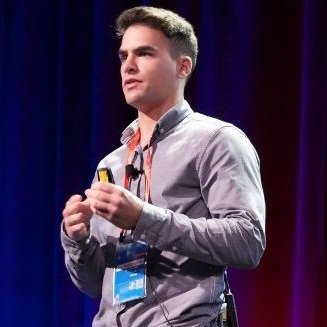
\includegraphics[scale=0.35]{avatar.jpg}} \\
\textsc{Degree:} & Master of Science in Computer and Telematics Engineering (2014) & \\
\textsc{Location:} & United States of America (born in Portugal) & \\
\textsc{Contacts:} & \href{mailto:igordcard+cv@gmail.com}{igordcard@gmail.com}  \href{mailto:igor.duarte.cardoso@intel.com}{igor.duarte.cardoso@intel.com} & \\
\textsc{Updated:} & September 2024 (\textbf{Public version 2024c.1}) & \\
\end{tabular} \\

%----------------------------------------------------
%	OBJECTIVES AND MOTIVATIONS
%----------------------------------------------------

\section{Professinal Summary}
I am passionate about designing solutions that prioritize user experience, thriving in collaborative environments:

\begin{itemize}
    \setlength{\itemsep}{1pt} % Reduce space between items
	\setlength{\parskip}{0pt}  % Reduce space between paragraphs (if needed)
	\setlength{\parsep}{0pt}   % Reduce space before and after list
	\item \textbf{Cloud Computing:} Experience with both open and closed-source projects.
	\item \textbf{Artificial Intelligence:} Eager to deepen my involvement in AI-driven projects.
	\item \textbf{Networking Technologies:} Expertise in Software-Defined Networking (SDN) and Network Functions Virtualization (NFV).
	\item \textbf{Hardware \& Server Management:} Ensuring robust system operations.
	\item \textbf{Cybersecurity:} Implementing secure solutions.
	\item \textbf{Mobile App Development:} Crafting user-centric applications.
\end{itemize}

I am particularly interested in roles where I can fully immerse myself in AI, contributing to projects that benefit from collective expertise and teamwork. My approach is always to enhance product development through collaborative efforts rather than working in isolation.


%----------------------------------------------------
%	WORK EXPERIENCE SUMMARY
%----------------------------------------------------

\section{Work Experience (summarized)}
\label{section:work_experience_summarized}
\begin{tabular}{r|p{13.4cm}}
	\emph{November 2024} & \textbf{AI Solutions Engineer} \\
	\textsc{February 2024} & Intel Corporation (Hillsboro, OR, United States of America) \\
	& \footnotesize{I was a founding member of an innovative team with the mission to develop a cutting-edge, production-ready AI datacenter cloud software stack. Our goal was to maximize the efficiency of Intel Gaudi AI accelerators on a massive scale. Despite our promising start, the project was ultimately discontinued due to financial constraints.}\\
	\multicolumn{2}{c}{} \\
	
	\emph{February 2024} & \textbf{Senior Cloud Orchestration Software Engineer }\\
	\textsc{November 2018} & Intel Corporation (Hillsboro, OR, United States of America) \\
	& \footnotesize{In reverse chronological order: Designed and developed features and solutions for a Cloud Security and Cloud Native project, for Intel Tiber Edge Platform, for Open-source EMCO (edge multi-cloud orchestrator) and Open-source Akraino (edge project). Lots of OpenStack, Kubernetes, Linux. Took roles such as EMCO TSC alternate chair, EMCO technical marketing rep, main point of contact for PM-related topics initiated by the EMCO open-source community at large.}\\
	\multicolumn{2}{c}{} \\
	
	\emph{November 2018} & \textbf{Network Software Engineer} \\
	\textsc{September 2015} & Intel Communications Europe (Shannon, Ireland) \\
	& \footnotesize{NFV, SDN, Service Function Chaining leadership in OpenStack, Open-source OpenStack contributions, hardware enablement and later solutions, including based on Intel Rack Scale Design.}\\
	\multicolumn{2}{c}{} \\
	
	\emph{September 2015} & \textbf{Researcher and Software Engineer} \\
	\textsc{October 2014} & Instituto de Telecomunicações (Aveiro, Portugal) \\
	& \footnotesize{NFV, SDN, telco vHGW/CPE, with the help of Open-source cloud computing (mainly OpenStack).}\\
	\multicolumn{2}{c}{} \\
	
	\emph{November 2015} & \textbf{Developer, Designer and Product Manager} \\
	\textsc{May 2013} & Wrkout (\textit{remote}, Portugal) \\
	& \footnotesize{Android mobile app with thousands of paying customers.}\\
	\multicolumn{2}{c}{}\\
	
	\emph{September 2012} & \textbf{Research Scholarship} \\
	\textsc{September 2011} &IEETA (University of Aveiro, Portugal) \\
	& \footnotesize{User Experience and Human-Computer Interfaces.}\\
	\multicolumn{2}{c}{}\\
	
\end{tabular}

%----------------------------------------------------
%	PATENTS
%----------------------------------------------------

\section{Patents}
\begin{enumerate}
	\item "Methods and apparatus to manage heat in a central processing unit", \href{https://patentimages.storage.googleapis.com/32/e3/4b/5e6bfda356c6f9/US11048540.pdf}{US11048540}, granted 2021
	\item (title hidden until publicly available) - on cloud native \& computer security, expected 2024
	\item (title hidden until publicly available) - on cloud native \& computer security, expected 2024
\end{enumerate}

Note: patent submissions turned into trade secrets will not be public and thus are not listed.

%----------------------------------------------------
%	ACHIEVEMENTS AND AWARDS
%----------------------------------------------------

\section{Achievements and Awards}

\begin{tabular}{rl}
	\textsc{2023} & Intel Security Leadership Award for my contributions to Cloud Burst Canyon. \normalsize\\
	\textsc{2022} & Intel Distinguished Invention Award in single-author patent work deemed trade secret. \normalsize\\
	\textsc{2021-22} & EMCO Technical Steering Committee alternate chair.\normalsize\\
	\textsc{2020-21} & Intel Recognition Award for work in EMCO, which I can't seem to dig up right now.\normalsize\\
	\textsc{2018} & Intel DSG DRA (Division Recognition Award) for my work in advancing IETF SFC and NSH. \normalsize\\
	\textsc{2017} & Intel DNSG DRA (Division Recognition Award) for my work in advancing IETF SFC and NSH. \normalsize\\
	\textsc{2017} & Intel Marketing DOT. \normalsize\\
	\textsc{2016} & Founded the CCF for Neutron in OpenStack, successfully bringing the community together. \normalsize\\
	\textsc{2016} & Intel DNSG recognition for co-organizing the first ever OpenStack Days Ireland event. \normalsize\\
	\textsc{2014} & Invited to develop a mobile Android app (ActUA) by the University's top staff. \normalsize\\
	\textsc{2013} & First place on a University's Mobile App Development challenge awarded by Blip.pt. \normalsize\\
	\textsc{2011} & Research Integration Scholarship (12-month) at IEETA, financed by FCT. \normalsize\\
	\textsc{2008} & Top (\#1) High School Student Award. \normalsize\\
\end{tabular} \\

%----------------------------------------------------
%	

%----------------------------------------------------

\section{Skills}

To keep the first 2 pages compact, detailed skill list has been moved to page 5.

%----------------------------------------------------
%       PUBLICATIONS
%----------------------------------------------------

\section{Publications}
\label{section:publications}
\begin{tabular}{rl}
	\textsc{2016} & Vitor Cunha, Igor D.C., J.P. Barraca, R.L. Aguiar: \\
	& ``Policy-driven vCPE through dynamic network service function chaining''. \\
	& NetSoft Conference and Workshops (NetSoft), 2016 IEEE, 156-160. \normalsize\\
	
	\textsc{2016} & Igor D.C., J.P. Barraca, Carlos Goncalves, R.L. Aguiar: \\
	& ``Seamless integration of Cloud and Fog networks''. \\
	& International Journal of Network Management 26 (6), 435-460. \normalsize\\
	
	\textsc{2015} & Igor D.C., J.P. Barraca, Carlos Goncalves, R.L. Aguiar: \\
	& ``Seamless integration of Cloud and Fog networks''. \\
	& 1st IEEE Conference on Network Softwarization (NetSoft 2015). \normalsize\\
	
	\textsc{2014} & Paulo Dias, Tiago Sousa, Joao Parracho, Igor D.C., André Monteiro, Beatriz Sousa Santos: \\
	& ``Student Projects Involving Novel Interaction with Large Displays''. \\
	& IEEE Computer Graphics and Applications, vol. 34, no. 2, pp. 80-86, Mar.-Apr., 2014. \normalsize\\
	
	\textsc{2014} & Tiago Sousa, Igor D.C., João Parracho, Paulo Dias, Beatriz Sousa Santos: \\
	& ``DETI-Interact: Interaction with Large Displays in Public Spaces Using the Kinect''. \\
	& HCI 2014 - 16th International Conference on Human-Computer Interaction: 196-206. \normalsize\\
	
	\textsc{2014} & Igor D.C.: \\
	& ``Network infrastructure control for virtual campuses''. \\
	& Universidade de Aveiro (Master's Dissertation). \normalsize\\
	
	\textsc{2013} & Tiago Sousa, João Parracho, Igor D.C., Paulo Dias, Beatriz Sousa Santos: \\
	& ``Interação com ecrãs de larga dimensão usando o kinect''. \\
	& Atas da 5ª Conferência Nacional sobre Interação-Interação. \normalsize\\
	
	\textsc{2012} & Igor D.C., Paulo Dias, Beatriz Sousa Santos: \\
	& ``Interaction with large displays in a public space using the Kinect sensor''. \\
	& 20 Encontro português de Computação Gráfica - EPCG 2012, pp. 81–88 (2012). \normalsize\\
	
\end{tabular} \\

\newpage

\begin{center} 
	\LARGE{For additional experience or greater detail, see pages below.}
\end{center} 

%----------------------------------------------------
%	WORK EXPERIENCE
%----------------------------------------------------

\section{Work Experience}
\label{section:work_experience}
\begin{tabular}{r|p{13.4cm}}
	\emph{November 2024} & \textbf{AI Solutions Engineer} \\
	\textsc{February 2024} & Intel Corporation (Hillsboro, OR, United States of America) \\
	& \footnotesize{I was a founding member of an innovative team with the mission to develop a cutting-edge, production-ready AI datacenter cloud software stack. Our goal was to maximize the efficiency of Intel Gaudi AI accelerators on a massive scale. Despite our promising start, the project was ultimately discontinued due to financial constraints.}\\
	\multicolumn{2}{c}{} \\
	
	\emph{February 2024} & \textbf{Senior Cloud Orchestration Software Engineer}\\
	\textsc{November 2018} & Intel Corporation (Hillsboro, OR, United States of America) \\
	& \scriptsize{Initially joined the Open Source Technology Center (OTC) with a focus on networking contributions to Neutron, the OpenStack networking project. Co-worked on Intel Omni-Path Architecture} testing and development/enabling in Neutron, joined in on existing miscellaneous OpenStack contribution work that was ongoing such as distributed virtual routing, virtual data path acceleration, and OVN, helping to close those by being an overall jack of all trades. Helped set up server hardware and development environments to optimize team performance and expectations. Contributed deployment and automation scripting to the Akraino edge project. Had brief exposure to the ONAP project, followed by the multi-k8s sub-project which eventually spun off to become EMCO, the Edge Multi Cloud Orchestrator, initiating my venture into Kubernetes and edge computing/orchestration. Contributed multiple features to EMCO, starting with multi-tenancy and ending with Google Anthos GitOps rendering support for apps deployed over Google Cloud. Throughout my time in EMCO, my software engineering role was raised to a senior level. Was named alternate TSC chair of EMCO by the TSC chair throughout most of 2021/2022, and was briefly part of the technical marketing team. I also mentored a student under the Linux Foundation mentorship program. After the EMCO investment wound down, I began working on Intel Tiber Edge Platform, contributed a significant chunk of a key component within Maestro-A, especially the multi-threaded state machine architecture that, as far as I'm aware, is still being used. Participated extensively in meetings about all parts of Maestro-A. After Tiber Edge, went on to work on Intel Cloud Burst Canyon, part of cloud native security and sustainability, contributing to a fundamental piece in the scheduling of applications with security requirements/expectations and created an IDF that is now pending patent submission. Finally, during my final time in this position, I have worked on ramping up in Intel TDX and a bit of IDC (Intel Developer Cloud) with the aim of accelerating TDX adoption (with Intel Amber attestation support) in IDC and provided extensive documentation about my findings and obstacles. As I was ramping up on Kubernetes KEDA (scaling), my team was defunded. Throughout these years I have earned some group awards and several recognitions from peers, managers and architects.\\
	\multicolumn{2}{c}{} \\

	\emph{November 2018} & \textbf{Network Software Engineer} \\
	\textsc{September 2015} & Intel Communications Europe (Shannon, Ireland) \\
	& \scriptsize{I have helped use cases and projects in the SDN, NFV and Orchestration areas on multiple occasions. Originally, I worked on the Group-Based Policy OpenStack project where I integrated QoS support from existing Neutron's APIs. Later, and during the majority of my time at Intel Communications Europe, I worked with SFC (Service Function Chaining). With a deep understanding of IETF SFC's proposal, architecture and the NSH protocol, I have fought through different obstacles in the OpenStack community in order to enable standards-compliant SFC, designing and proposing a compatible solution. I later implemented SFC Encapsulation support for OpenStack's Neutron (networking-sfc) through multiple patches, mainly the ones enabling Service Graphs and the NSH protocol (for Open vSwitch), and became part of the core team. Additionally, I have designed, developed and successfully contributed an abstract SFC interface for the VIM connector layer in the Open Source MANO (OSM) project, together with an OpenStack implementation of it, and enabled ETSI NSD/VNFFGD to be converted to the VIM connector's SFC interface, thus enabling top-to-bottom, end-to-end SFC from orchestration all the way down to Open vSwitch (optionally together with OpenDaylight), all based on open source projects. Another very significant endeavour was resurrecting the effort around traffic classification in OpenStack's Neutron, by founding and leading the Common Classification Framework project, creating an initial design and bringing the community together to discuss, suggest and agree on use cases and models. Most recently, I began working with Intel Rack Scale Design (RSD), where I have provided contributions on a diverse set of layers. My most tangible contribution in RSD is the inception of the \verb+rsb_+ module umbrella and the creation of the \verb+rsd_node+ module, allowing Ansible to deploy composed nodes in an idempotent manner. Finally, I've worked on multiple innovation tasks during my time.}\\
	\multicolumn{2}{c}{} \\

	\emph{September 2015} & \textbf{Researcher and Software Engineer} \\
	\textsc{October 2014} & Instituto de Telecomunicações (Aveiro, Portugal) \\
    & \scriptsize{Given the experience I acquired in OpenStack during my Master's Dissertation and the related work I did during it, I was invited to stay at Instituto de Telecomunicações doing research related to Network Functions Virtualization (NFV). There, I kept working on OpenStack although initially not upstream. Then started making contributions to the Group-Based Policy project for OpenStack. Most of my work, though, has been around other aspects of NFV: automating configuration of Virtual Network Functions (VNFs), improving and discussing the Traffic Steering implementation to meet the purposes of Service Function Chaining (SFC), testing and integrating other implementation artifacts of the team. }\\
	\multicolumn{2}{c}{} \\

	\emph{November 2015} & \textbf{Developer, Designer and Product Manager} \\
	\textsc{May 2013} & Wrkout (\textit{remote}, Portugal) \\
	& \scriptsize{Not really a job, but an amazing work experience. Wrkout is a mobile Android app which I've created. By dealing with multiple aspects related to developing, publishing and monetizing the app by myself, I have learned plenty. This project turned product also teaches me exactly why I should be working in a team. Wrkout also gave me the first non-college exposure to software product management, as I took customer requirements and iterated over those alongside my long-term vision for the app. On November 2015 the app was made free and I became less engaged with it in order to better focus on my new endeavours.}\\
	\multicolumn{2}{c}{}\\
	
	\emph{September 2012} & \textbf{Research Scholarship} \\
	\textsc{September 2011} &IEETA (University of Aveiro, Portugal) \\
	& \scriptsize{In this part-time scholarship awarded by merit during university, I got introduced to the world of academic research for the first time. Here I developed solutions in the area of user interfaces, user experience and human-computer interfaces. I was able to get acquaint myself with Microsoft Kinect, Oculus Rift, 3D sensing and modeling, UI Testing, and refine my existing C\# and Visual Studio skills. The developments led to publications and one public speaking engagement at a conference.}\\
	\multicolumn{2}{c}{}\\

\end{tabular}


%----------------------------------------------------
%	SKILLS
%----------------------------------------------------

% -- TensorFlow, Deep Learning, Neural Networks, LLMs
% -- Ray (next to KubeRay)
% - SPIFFE/SPIRE, KEDA

\section{Skills}

\begin{tabular}{rl}
	Basic Experience:
	& Ansible, ASP.NET, bison, C, C++, Computer Architecture, Dansguardian,\\
	& flex, iOS dev, Jekyll, MIPS assembly, Objective-C, OpenDaylight,\\
	& OpenWrt, OSM, Perl, PHP, Ruby, Squid3, x86 assembly, SMO, AI/ML/DL,\\
	& GKE, Anthos, Heroku, MongoDB, Akraino, GitOps, Kyverno, Intel TDX,\\
	& Microsoft Project, Marketing, Product Management, \\
	& Hugging Face, PyTorch, MPI, Ray, SPIFFE/SPIRE, KEDA, Intel Gaudi.\\
	Intermediate Experience:
	& Android dev, bash, C, C\#, Cisco IOS, CSS, ETSI NFV, Excel, \\
	& GlassFish, GNS3, GNU/Linux, Google Analytics, HTML, IETF SFC/NSH \\
	& Intel Rack Scale Design, Java, JavaScript, Jenkins, LAMP, {\LaTeX}, \\
	& Computer Networks, Computer Security, Neutron, OpenFlow,\\
	& OpenStack, Open vSwitch, Public Speaking, golang,\\
	& EMCO, Helm, project management, Distributed Systems, CI, \\
	& Python, Redfish, SQL, Technical Writing, UML, Vim, Visio, XML,\\
	& Wireshark, Software Architecture, Mentoring, Jupyter, KubeRay,\\
	& Video editing.\\
	Advanced Experience:
	& APIs, docker, git, JSON, JIRA, Linux dev environments, VSCode,\\
	& Microservices, Kubernetes.
\end{tabular} \\


%----------------------------------------------------
%	EDUCATION
%----------------------------------------------------

\section{Formal Education}

\begin{tabular}{rl}
    \textsc{2014} & Master of Science in \textsc{Computer and Telematics Engineering}, \\
    &\textbf{Universidade de Aveiro}, Aveiro, Portugal, \\
    & Dissertation: ``\href{https://ria.ua.pt/bitstream/10773/14707/1/Controlo%20de%20Infrastrutura%20de%20Rede%20para%20Campus%20Virtuais.pdf}{Network Infrastructure Control for Virtual Campus}", \\
    & Based on a broad Computer Science foundation, further focuses on Software Engineering\\
    & and Computer Networks.\\
    & \textit{Final grade: 18 out of 20 (dissertation).}\\
    &\\
    
     \textsc{2011} &  Bachelors in \textsc{Computer and Telematics Engineering}, \\
    &\textbf{Universidade de Aveiro}, Aveiro, Portugal, \\
    & Degree with a broad Computer Science foundation (linear algebra included)\\
    & and multiple practical projects.\\
    & \textit{Final grade: 16 out of 20.}\\
    &\\

    \textsc{2008} & High School, \\
    &\textbf{Agrupamento de Escolas da Guia}, Guia, Portugal: \\
    & \textit{Final grade: 18 out of 20 (top of class).}\\
    &\\
\end{tabular}

%----------------------------------------------------
%	MASTERS DISSERTATION
%----------------------------------------------------
\subsection{Master's Dissertation}
On my Master's Dissertation I have designed and developed an extension for OpenStack Neutron that allows virtually any computer network to be extended beyond their physical boundaries up to a Cloud-managed network, per a Cloud tenant's request. This is achieved through an architecture that uses pluggable drivers to communicate with remote devices that directly connect or manage these computer networks.

%----------------------------------------------------
%	NON-FORMAL EDUCATION
%----------------------------------------------------
\subsection{Non-formal education}
\begin{itemize}
    \item Cisco CCNA-1 - 2007.
    \item Public Speaking course (1 day) - 2016.
    \item Crucial Conversations and Conflict Resolution course (1 day) - 2017.
%    \item Career Empowerment Program (2 days) - 2019.
    \item Bitnami Kubernetes training (CKA+CKAD-like) (3 days) - 2019.
    \item Ardan Labs Ultimate Go training (2 days) - 2019.
\end{itemize}

\newpage

%----------------------------------------------------
%	PUBLIC PRESENTATIONS
%----------------------------------------------------

\section{Public Presentations}
Presentation on human-computer interaction\\
Viana do Castelo, Portugal, 2012

Presentation on 24-hour mobile app hackaton\\
Lisbon, Portugal, 2013

\href{https://www.slideshare.net/igordcard/empower-your-nfv-services-through-service-function-chaining-and-sfc-graphs}{Empower your NFV Services through Service Function Chaining and SFC Graphs}\\
OpenStack Summit 2016, Barcelona

\href{https://www.slideshare.net/igordcard/developing-deploying-and-consuming-l47-network-services-in-an-openstack-cloud}{Developing, Deploying, and Consuming L4-7 Network Services in an OpenStack Cloud}\\
OpenStack Summit 2016, Austin, Texas

\href{https://www.slideshare.net/igordcard/cloud-sdn-nfv}{Cloud, SDN, NFV}\\
ENEI 2016, University of Aveiro, Portugal

\textit{\href{https://www.slideshare.net/igordcard/cloud-sdn-nfv}{On Intel OPA} (submission was accepted but travel was not approved)}\\
Open Infrastructure Summit 2019,  Shanghai, China

\href{https://wiki.lfnetworking.org/pages/viewpage.action?pageId=65537697}{EMCO: Deploying to target clusters (and public clouds) via git}\\
LFN DTF June 2022, Porto, Portugal

\href{https://wiki.lfnetworking.org/pages/viewpage.action?pageId=65537697}{EMCO: distribution of Istio CA certificates to target clusters} (on behalf of 3rd party)\\
LFN DTF June 2022, Porto, Portugal

\href{https://wiki.lfnetworking.org/pages/viewpage.action?pageId=65537697}{Project Overview and Update} (on behalf of 3rd party)\\
LFN DTF June 2022, Porto, Portugal

\href{https://gitopsconna22.sched.com/event/1AR8V}{Simplifying Edge Deployments Using EMCO and GitOps}\\
KubeCon North America 2022, Detroit, Michigan\\

%----------------------------------------------------
%	Open-Source Output
%----------------------------------------------------

\section{Open-Source Output}
I have made upstream contributions to a diverse set of projects within the OpenStack umbrella.

I have made other contributions to Open-Source software that are public but not all of them upstream, including irssi, Yakuake, metastore, tox, etc. I have also developed other simple side projects in the past, some of them available at my GitHub.

You can check most of my public output through the links/profiles/dashboards/pages below:
\begin{itemize}
    \item \href{https://review.openstack.org/#/q/owner:igordcard}{OpenStack Gerrit} and \href{https://review.openstack.org/#/q/owner:igordc}{new one}
    \item \href{http://stackalytics.com/?user_id=igordcard&metric=marks&release=all}{OpenStack Stackalytics} and \href{http://stackalytics.com/?user_id=igordc&metric=marks&release=all}{new one}
    \item \href{https://osm.etsi.org/gerrit/#/q/owner:cardosoi}{OSM Gerrit}
    \item \href{https://wiki.openstack.org/wiki/Neutron/CommonClassificationFramework}{CCF Wiki}
    \item \href{https://launchpad.net/~igordcard}{Launchpad Profile}
    \item \href{https://github.com/igordcard}{GitHub Profile}
    \item \href{https://gitlab.com/igordc}{GitLab Profile}
\end{itemize}

%----------------------------------------------------
%	PRESENCE
%
% This section will deal with both my presence on the web (how to reach me, by professional profiles, etc)
% as well as my presence regardings groups, associations, development teams, open source projects, etc.
%----------------------------------------------------

\section{Presence}
\begin{tabular}{r|p{11cm}}
    \emph{ATNoG} & Advanced Telecommunications and Networks Group \\
    \textsc{September 2013} & \footnotesize{I became associated with ATNoG as part of my Master's Thesis. This group is established inside Aveiro's pole of Instituto de Telecomunicações.}\\
    \multicolumn{2}{c}{} \\
    \emph{GLUA} & University of Aveiro's Linux Group \\
    \textsc{July 2011} & \footnotesize{Member of the University of Aveiro's Linux Group (Grupo Linux da Universidade de Aveiro).}\\
    \multicolumn{2}{c}{}\\
\end{tabular}

%----------------------------------------------------
%	EVENTS
%----------------------------------------------------

\section{Events}
\begin{tabular}{r|p{11cm}}
    \emph{As a co-organizer} & OpenStack Days Ireland 2016 \\
\end{tabular} \\

%----------------------------------------------------
%	INTERESTS AND ACTIVITIES
%----------------------------------------------------

\section{Interests and Activities}
Computer Software, 
Computer Hardware, 
Cloud Computing, 
GNU/Linux, 
Open-Source, 
Computer Networks, 
Brainstorming, 
User Experience, 
Health and Fitness, 
Brazillian Jiu-Jitsu, 
Reading, 
Artificial Intelligence.

%----------------------------------------------------
%	LANGUAGES
%----------------------------------------------------

\section{Languages}

\begin{tabular}{rl}
	\textsc{Portuguese:} & Native\\
	
	\textsc{English:} & Fluent\\
	
	\textsc{Spanish:} & Basic understanding\\
	
\end{tabular} \\

%----------------------------------------------------
%	ADDITIONAL NOTES
%----------------------------------------------------

%\section{Additional Notes}
%\begin{itemize}
%	\item Co-pioneer of <the box project>  add once ready
%\end{itemize}

\end{document}
